\section{Introduction}
\label{sec:chapter_1_2_introduction}
\subsection{Definitions}
\begin{itemize}
	\item The quantified self can be defined as:
	\blockquote{\textit{The quantified self is any individual engaged in the self-tracking of any kind of biological, physical, behavioral, or environmental information. \\The self-tracking is driven by a certain goal of the individual with a desire to act upon the collected information.}}
	\item \textbf{Augemberg} (2012): there are various types of measurements, including:
	\begin{itemize}
		\item Physical activities (movement by accelerometer, steps, etc.)
		\item Diet (calories consumed, fat, protein, etc.)
		\item Psychological states (mood, emotions, depression, etc.)
		\item Mental and cognitive traits (IQ, reaction, memory, etc.)
		\item Environmental (location, weather, etc.)
		\item Situational (time of the day, context, etc.)
		\item Social variables (influence, role in a group, etc.)
	\end{itemize} 
	\item \textbf{Choe} (2014): distinguish quantified selves into three categories based on their goal.
	\begin{itemize}
		\item Improved health (cure or manage a condition,
		execute a treatment plan, achieve a goal)
		\item Improve other aspects of life (maximize work performance, be mindful)
		\item Find new life experiences (have fun, learn new things)	
	\end{itemize}
	\item \textbf{Gimpel} (2013): identified five (non-exclusive) factors for quantified self motivation
	\begin{itemize}
		\item Self-healing (to become healthier)
		\item Self-discipline (to experience rewarding aspects of it)
		\item Self-design (to control and optimize ``yourself'', as e.g. on sport)
		\item Self-association (to be associated with the movement of QS)
		\item Self-entertainment (to experience entertainment value)
	\end{itemize}
	\item Machine Learning (automatically identifying patterns from data) is slightly different in the setting of Quantified Self because
	\begin{itemize}
		\item we have to deal with sensory noise
		\item there might be missing measurements
		\item we have temporal data (feature engineering) with irregular time points
		\item there can be an interaction with a user (advice for training/mood improvements, etc.), but we cannot try out every possibility
		\item Learn across multiple datasets/users
	\end{itemize}
	\item \comment{Most of the above definitions need to be memorized for the exam}
\end{itemize}
\subsection{Basic Terminology and Notation}
\begin{itemize}
	\item Measurement $=$ one value for an attribute recorded at a specific time point
	\item Time series $=$ series of measurements in temporal order
	\item Further notation: 
	\begin{itemize}
		\item For matrix $\bm{X}$, the columns are the different measurements like accelerometer, and rows are the time points (if dataset is temporally ordered, otherwise random list) 
	\end{itemize}
	\begin{figure}[ht!]
		\centering
		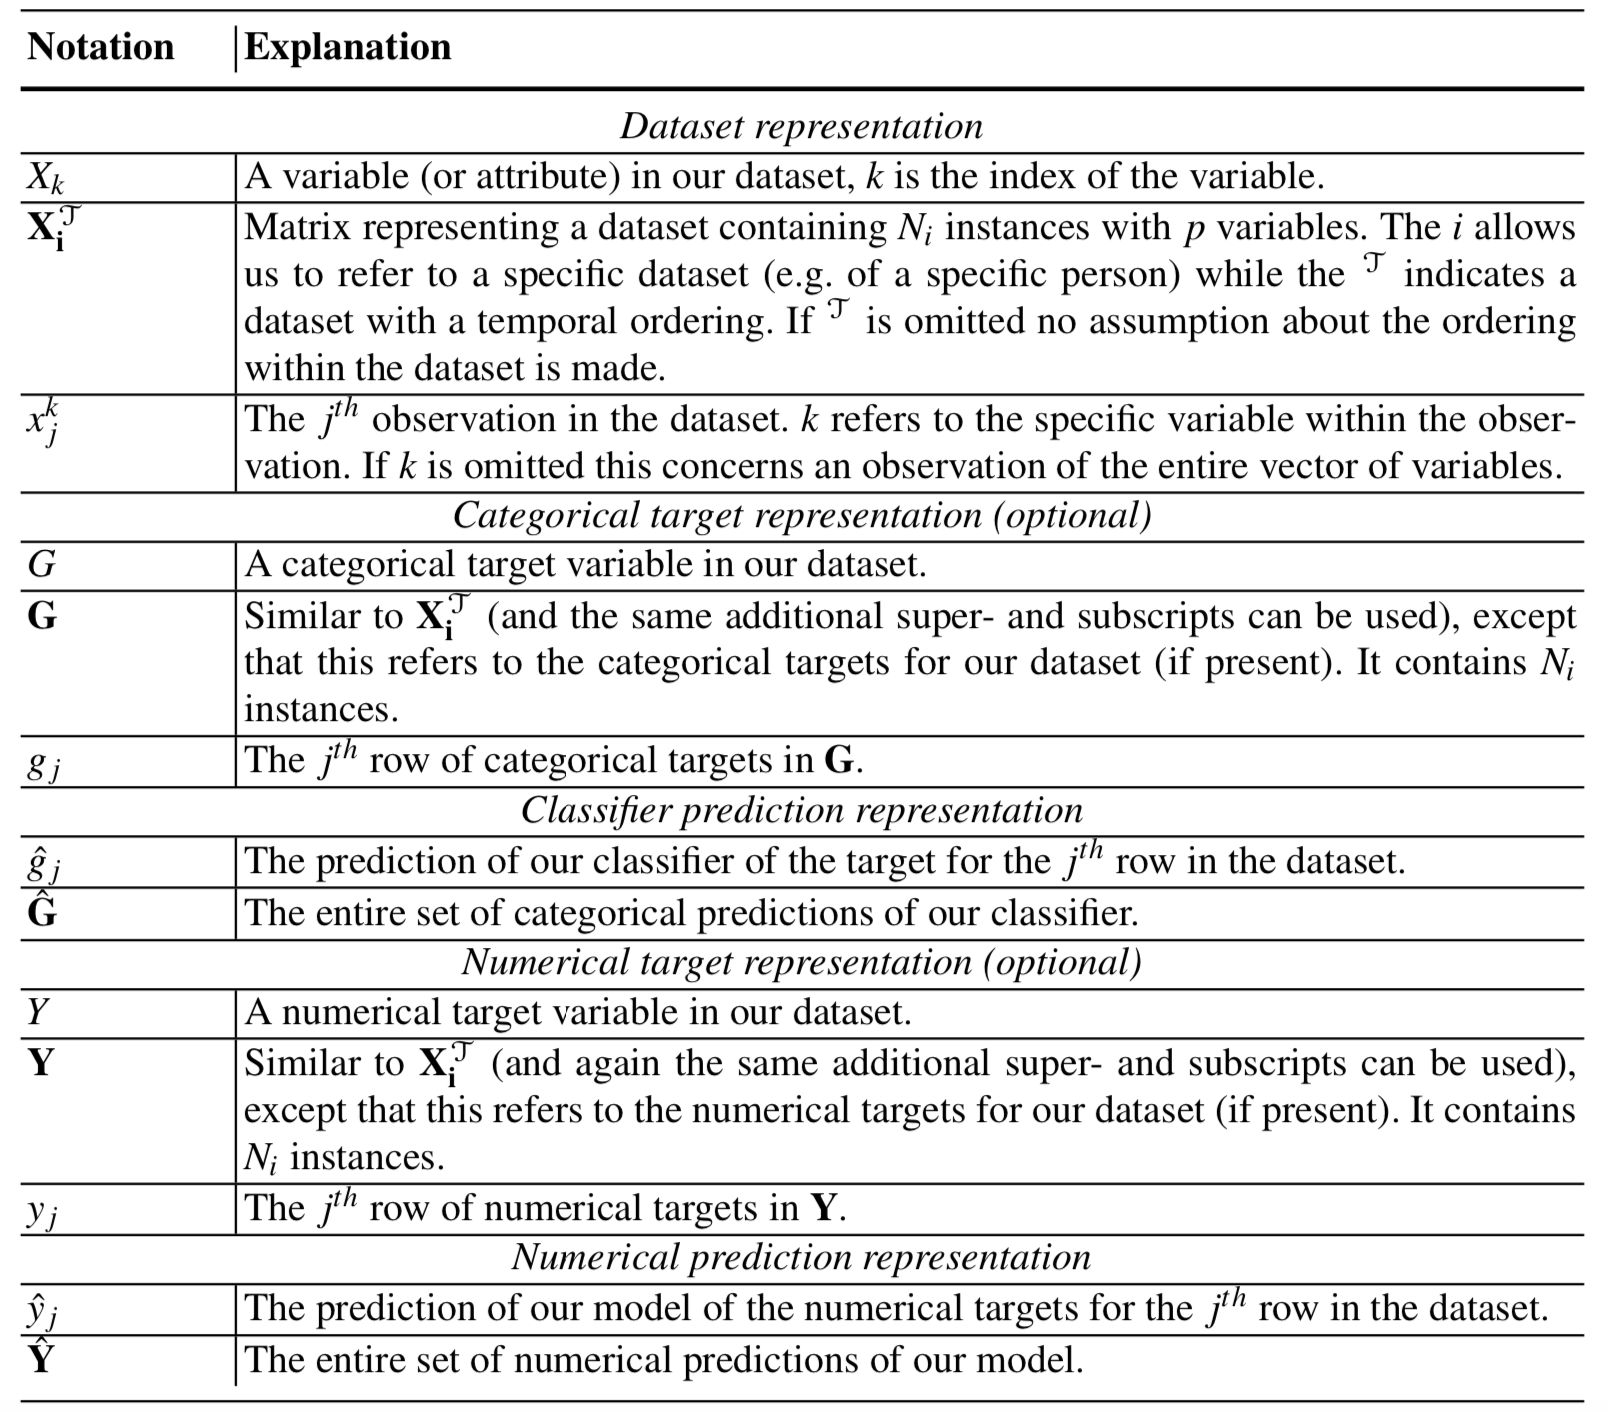
\includegraphics[width=0.4\textwidth]{figures/intro_notation.png}
		\caption{Overview of notation used in this course.}
	\end{figure}
\end{itemize}
\subsection{Basic overview of Sensory Data}
\begin{itemize}
	\item Different sensors available on mobile devices, such as:
	\begin{itemize}
		\item \textit{Accelerometer}: Measures the changes in forces upon the phone in the $x$-$y$-$z$ plane
		\item \textit{Gyroscope}: Orientation of the phone compared to
		the earth's surface
		\item \textit{Magnetometer}: Measures $x$-$y$-$z$ orientation compared to the earth's magnetic field
	\end{itemize}
	\item Transforming raw data of time series require selecting a step size $\Delta t$, and combine sensory data over this interval. See Section~\ref{sec:chapter_4_feature_engineering} for techniques
	\item A large $\Delta t$ gives (maybe too) coarse-grained data, but we have in the end a smaller dataset and lower standard deviation. The opposite is gained by a smaller $\Delta t$ (fine-grained data, but large dataset and high stddev)
\end{itemize}